\section{O Processador}

Esta seção irá descrever de forma geral a arquitetura do processador utilizado, o código fonte esta disponível em:

\url{https://github.com/felipe-samuel/Processador-Verilog}

\subsection{Visão Geral da Arquitetura}  

A arquitetura do processador utilizado possui um conjunto de instruções reduzidas,
similar ao MIPs possuindo apenas 28 instruções, cada uma com o tamanho de
32 bits, possui uma arquitetura load/store.

Possui um funcionamento monociclo, ou seja executará uma instrução a
cada ciclo de clock.

O processador pode ser dividido em duas Unidade, uma de controle, e outra de processamento, nas Figuras 1 e 2, os elementos pertencentes a estas unidades aparecem com as cores vermelha e azul, respetivamente.


\begin{figure}[!htb]
\begin{center}
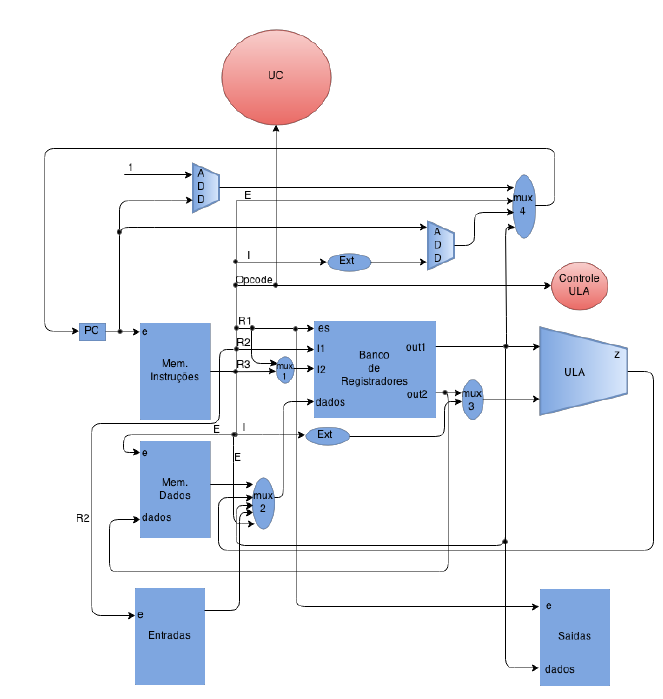
\includegraphics[scale=0.9]{figuras/Diagrama_da_cpu.jpeg} 
\end{center}
\caption{Diagrama da CPU}
\end{figure}


\begin{figure}[!htb]
\begin{center}
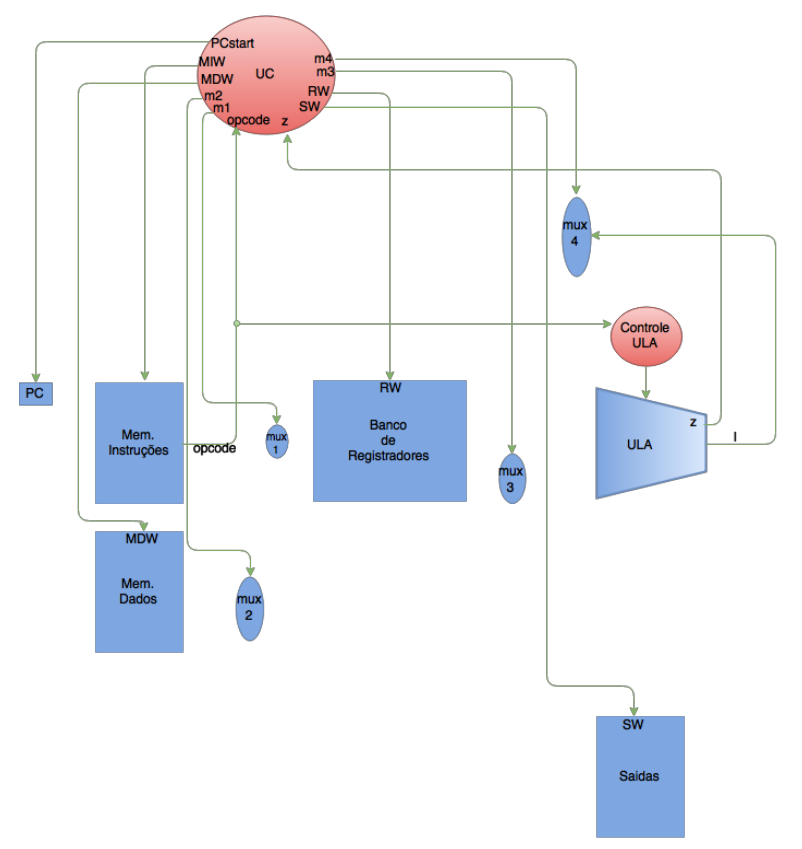
\includegraphics[scale=0.7]{figuras/Diagrama_dos_sianais_de_comtrole_da_cpu.jpeg} 
\end{center}
\caption{Diagrama dos Sinais de Controle da CPU}
\end{figure}

\subsection{Elementos da Unidade de Processamento}
A unidade de processamento possui os seguintes elementos.

\begin{itemize}

\item \textbf{Program Counter (PC):} Registrador de 22 bits que armazena, o endereço da instrução que está sendo executada na memória de instruções.

\item \textbf{Unidade Lógica Aritmética (ULA):} Tem a função de realizar operações lógicas e aritméticas e comparações (maior, menor, igual e diferente).

Tem duas entradas de dados de 32 bits, que definem os dois operandos, e uma entrada de controle de 4 bits, que define que operação será realizada, e 2 saídas, uma de 32 bits, que é o resultado de operações aritméticas e lógicas, e a saída de 1 bit L, que é o resultado de comparações (0 para falso e 1 para verdadeiro).

\item \textbf{Memória de Instruções: }Trata-se de uma memória vetorial com capacidade de armazenar 4194304 instruções de 32 bits.
Possui uma entrada (EMI), que é o endereço no vetor no qual o dado qual ocorrerá uma escrita de dados, ou será devolvido em sua saída de 32 bits.

A entrada de controle MIW define se haverá escrita ou não. 

\item \textbf{Memória de Dados:} Armazena dados de 32 bits, funcionamento igual a memória de instruções.

\item \textbf{Banco de Registradores:} Vetor de 32 registradores, possui 3 entradas, RE (Endereço do registrador em que ocorrerá a escrita de dados), RL1 (endereço do registrador cujo conteúdo será devolvido na saída Rout1 de 32 bits), RL2 (endereço do registrador cujo conteúdo será devolvido na saída Rout2 de 32 bits).

\item \textbf{Unidade de Entradas:} Vetor de 32 registradores, cada um de 32 bits, que armazenam o valor de dispositivos de entradas conectados a ele de forma síncrona com o sinal de clock, a entrada e tem a função de fazer a selecionar qual dos registradores será devolvido como saída.

\item \textbf{Unidade de Entradas:} Vetor de 32 registradores, cada um de 32 bits, que armazenam o valor de dispositivos de entradas conectados a ele de forma síncrona com o sinal de clock, a entrada e tem a função de fazer a selecionar qual dos registradores será devolvido como saída.

\item \textbf{Unidade de Saídas:} Vetor de 32 registradores, armazena valores de saídas que podem ser lidos por dispositivos externos, a entrada e tem a função de realizar a seleção sobre em qual registrador será escrito o valor da entrada dados.

O sinal de controle SW define se haverá escrita durante este ciclo de clock.


\item \textbf{Somadores (ADD):} Somam os dois valores de suas entradas;

\item \textbf{Extensores de Bits (Ext):} Aumentam a quantidade de bits do sinal de entrada acrescentando zeros.

\item \textbf{Multiplexadores (m):} De acordo com o sinal de controle recebido, a saída será igual a uma de suas entradas.

Controle da ULA: Recebe o Opcode como entrada, e define qual operação a ULA terá de realizar.

\end{itemize}

\subsection{Elementos da Unidade de Controle}

\begin{itemize}

\item \textbf{Unidade de Controle Geral (UC):} Trata-se de uma máquina de estado, que recebe como entrada o Opcode, e tem como saída diversos sinais de controle, que controlam a escrita de dados nas memória, banco de registadores, entradas e saídas, e o funcionamento dos multiplexadores. 

\item \textbf{Unidade de Controle da ULA:} Recebe o Opcode, e determina qual operação a ULA deverá realizar durante aquele ciclo de clock.

\end{itemize}



\subsection{Formato de Instruç\~oes}

Serão aceito 3 formatos diferentes de instruções.

\begin{itemize}

\item Formato 1:
\begin{tabular}{|c|c|c|c|c|}
\hline
Opcode[31:27] & R1[26:22] & R2[21:17] & R3[16:12] & -[11:0]\\
\hline
\end{tabular}


\item Formato 2:
\begin{tabular}{|c|c|c|c|}
\hline
Opcode[31:27] & R1[26:22] & R2[21:17] & I/-[16:0]\\
\hline
\end{tabular}

\item Formato 3:
\begin{tabular}{|c|c|c|}
\hline
Opcode[31:27] & R1/-[26:22] & E/-[21:0]\\
\hline
\end{tabular}

\end{itemize}

\subsection{Conjunto de Instruç\~oes}

A tabela 2 a seguir lista o conjunto de instruções que o processador é capaz de realizar.

\begin{table}[!htb]
\centering
\caption{Conjunto de Instruções}


\begin{tabular}{|c|c|c|c|}
 
\hline
\textbf{Opcode} & \textbf{Instrução} & \textbf{Funcionamento} & \textbf{formato}\\
\hline 

\multicolumn{4}{|c|}{\textbf{Operações aritiméticas}}\\

\hline 
00000 & Add[R1,R2,R3]  & $[R1]<= [R2] + [R3]$ & 1\\
\hline 
00001 & AddI[R1,R2,I]  & $[R1]<= [R2] + I$    & 2\\
\hline 
00010 & Sub[R1,R2,R3]  & $[R1]<= [R2]–[R3]$   & 1\\
\hline 
00011 & SubI[R1,R2,I]  & $[R1]<= [R2] - I$    & 2\\
\hline 
00100 & Mult[R1,R2,R3] & $[R1]<= [R2] * [R3]$ & 1\\
\hline 
00101 & MultI[R1,R2,I] & $[R1]<= [R2] * I$    & 2\\

\hline
\multicolumn{4}{|c|}{\textbf{Operações lógicas e de comparação}}\\
\hline

00110 & And[R1,R2,R3]  & $[R1]<= [R2] and [R3]$   & 1\\
\hline 
00111 & AndI[R1,R2,I]  & $[R1]<= [R2] and I$      & 2\\
\hline 
01000 & Or[R1,R2,R3]   & $[R1]<= [R2] or [R3]$    & 1\\
\hline 
01001 & OrI[R1,R2,I]   & $[R1]<= [R2] or I$       & 2\\
\hline 
01010 & Not[R1,R2]     & $[R1]<= NOT([R2])$       & 2\\
\hline 
01011 & Slt[R1,R2,R3]  & $[R1]<= 1, Se [R2]<[R3]$ & 1\\ && $[R1]<= 0, Se [R2]>= R3$ &\\
\hline 
01100 & SltI[R1,R2,I]  & $[R1]<= 1, Se [R2]< I $ & 2\\ && $ [R1] <= 0, Se [R2]>= I$   &\\

\hline
\multicolumn{4}{|c|}{\textbf{Operações de deslocamento de bits}}\\
\hline

01101 & Sll[R1,R2] & $[R1]<= SLL([R2])$  & 2\\
\hline 
01110 & Slr[R1,R2] & $[R1]<= SLR([R2])$  & 2\\

\hline
\multicolumn{4}{|c|}{\textbf{Operações de tranferências de dados}}\\
\hline

01111 & Move[R1,R2] & $[R1]<=[R2]$ & 2\\

\hline
\multicolumn{4}{|c|}{\textbf{Operações de saltos}}\\
\hline

10000 & J[E]         & $PC<=E$                       & 3\\
\hline 
10001 & Jr[R1]       & $PC<=[R1]$                    & 3\\
\hline 
10011 & Beq[R1,R2,I] & $PC<=PC + I, Se [R1] = [R2]$  & 2\\
\hline 
10100 & Bnq[R1,R2,I] & $PC<=PC + I, Se [R1] != [R2]$ & 2\\
\hline 
10101 & Bob[R1,R2,I] & $PC<=PC + I, Se [R1] > [R2]$  & 2\\
\hline 
10110 & Bos[R1,R2,I] & $PC<=PC + I, Se [R1] < [R2]$  & 2\\


\hline
\multicolumn{4}{|c|}{\textbf{Operações de acesso a memória interna}}\\
\hline

10111 & Load[R1,E]  & $[R1]<=RAM\_DADOS(E)$ & 3\\
\hline 
11000 & Store[R1,E] & $RAM\_DADOS(E)<=[R1]$ & 3\\

\hline
\multicolumn{4}{|c|}{\textbf{Operações de acesso as entradas e saídas}}\\
\hline

11001 & Input[R1,R2]  & $[R1]<=ENT(R2)$    & 2\\
\hline 
11010 & Output[R1,R2] & $SAIDAS(R1)<=[R2]$ & 2\\

\hline
\multicolumn{4}{|c|}{Outras}\\
\hline

11011 & SetR[R1,E] & $[R1]<=E$ & 3\\
\hline
11111 & End[\ \ ]      & $PC<=PC $ & 3\\
\hline

\end{tabular}

\end{table}


\clearpage